\subsection{InGame - Interface}

\subsubsection{tick.Tick}

\begin{center}
    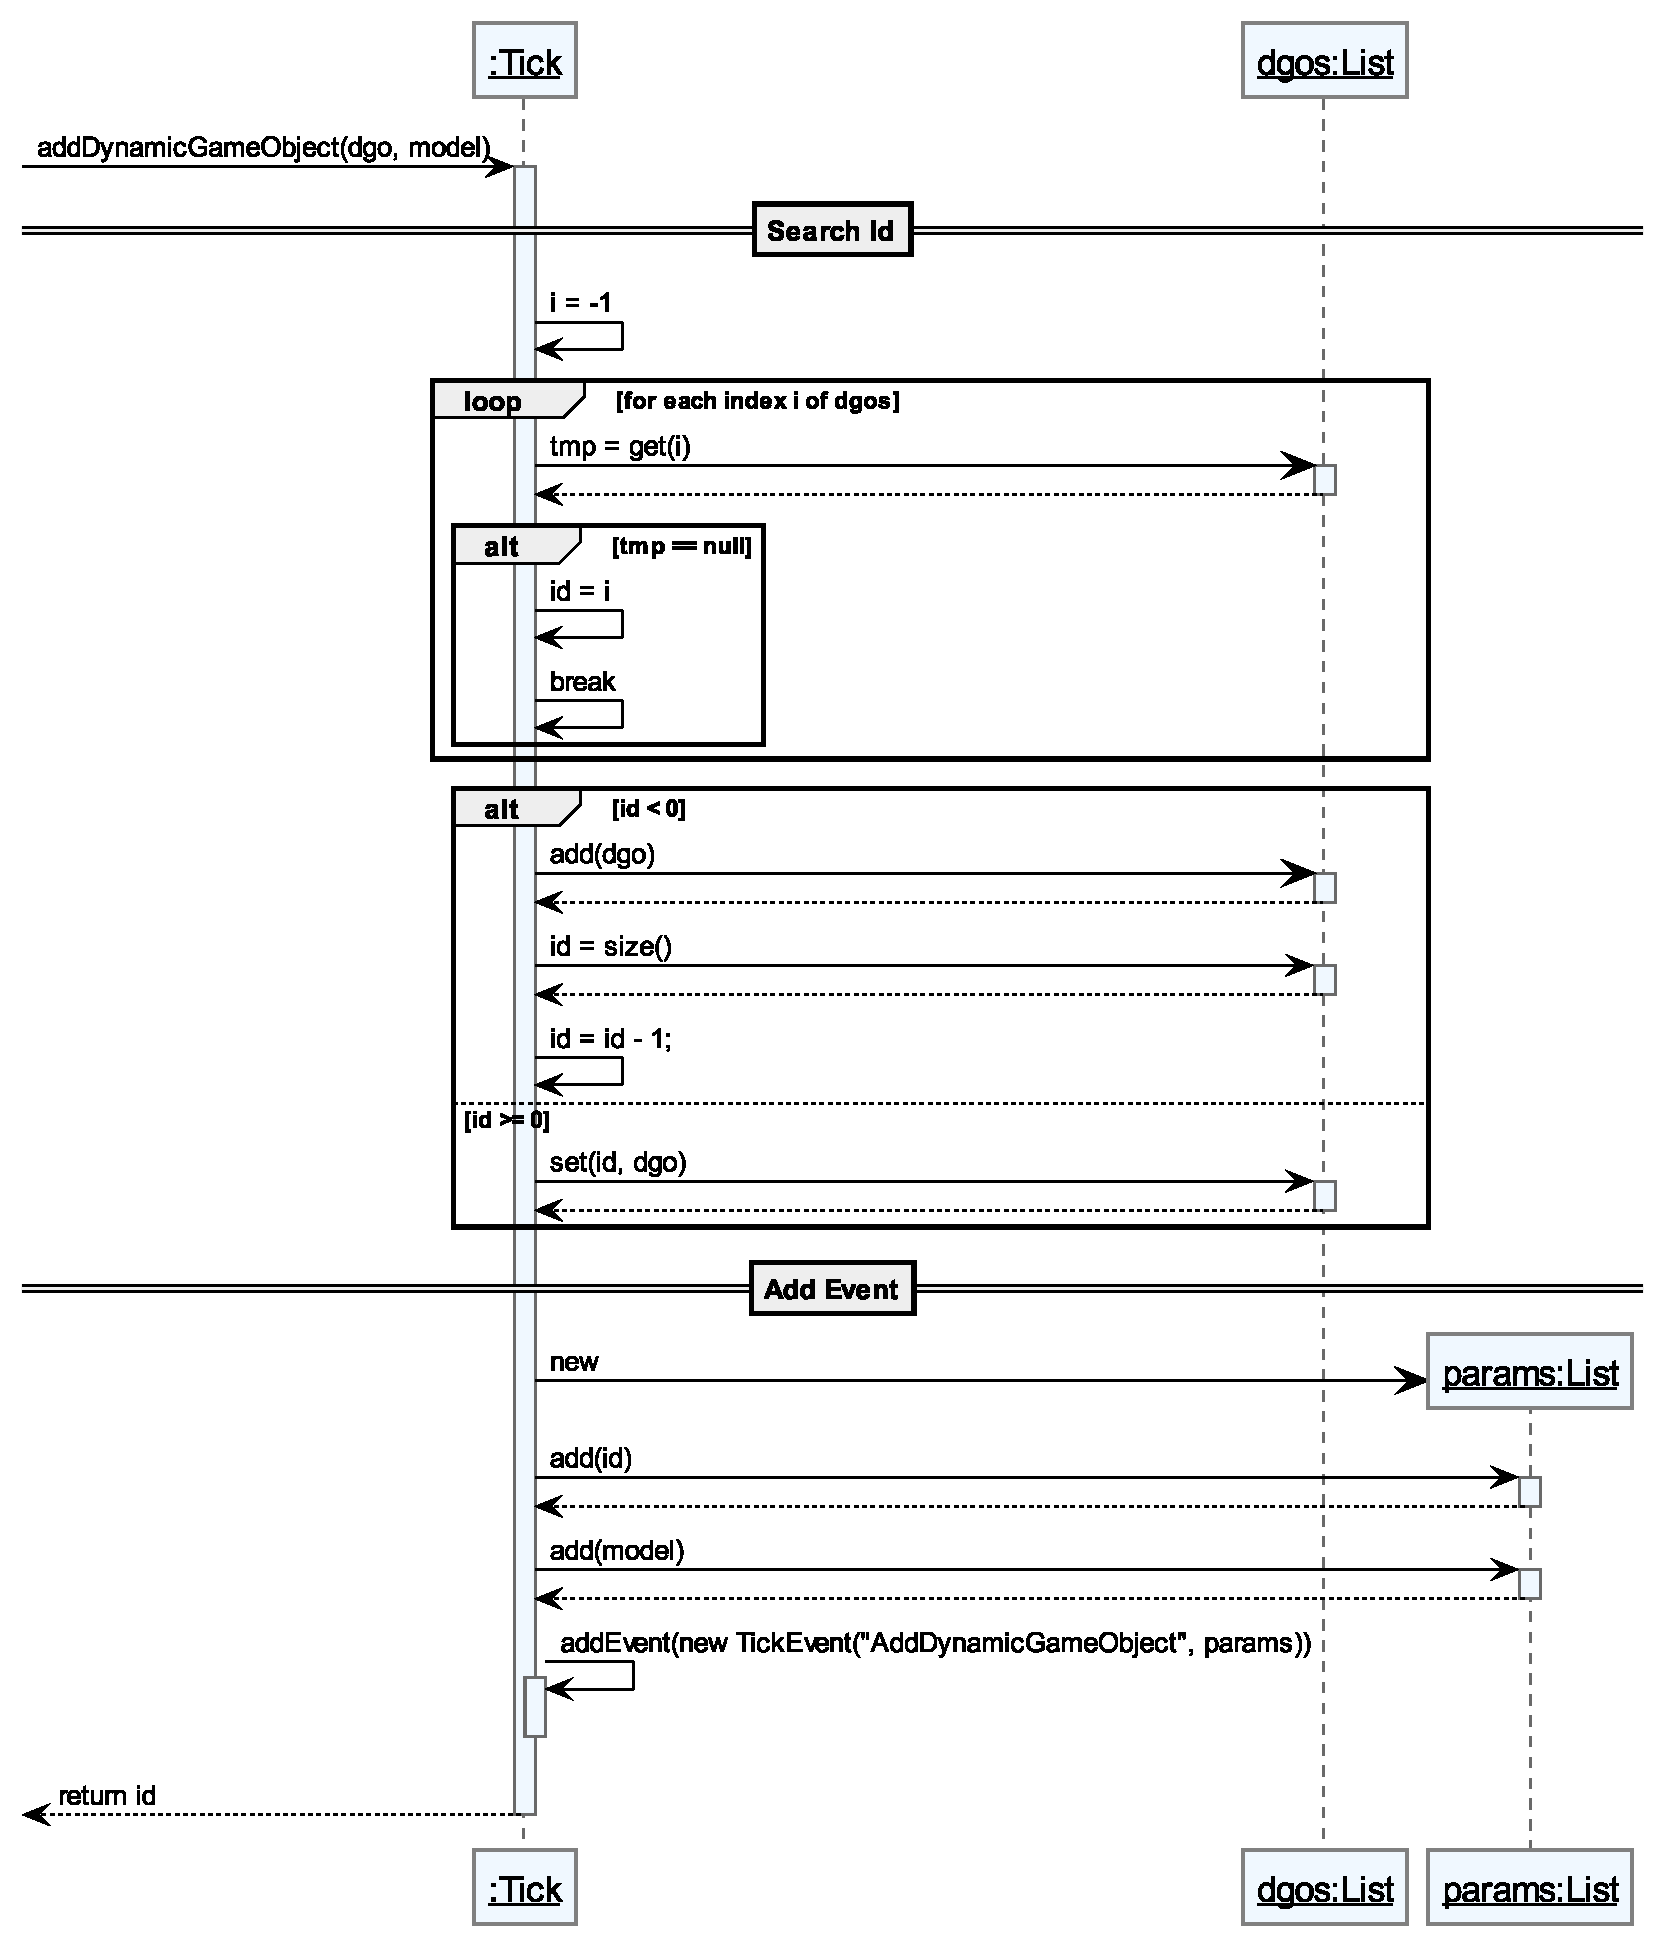
\includegraphics[width=\linewidth]{Interface/Tick_addBundle.eps}
    \captionof{figure}{Tick.addDynamicGameObject()}
\end{center}

\begin{center}
    \centering
    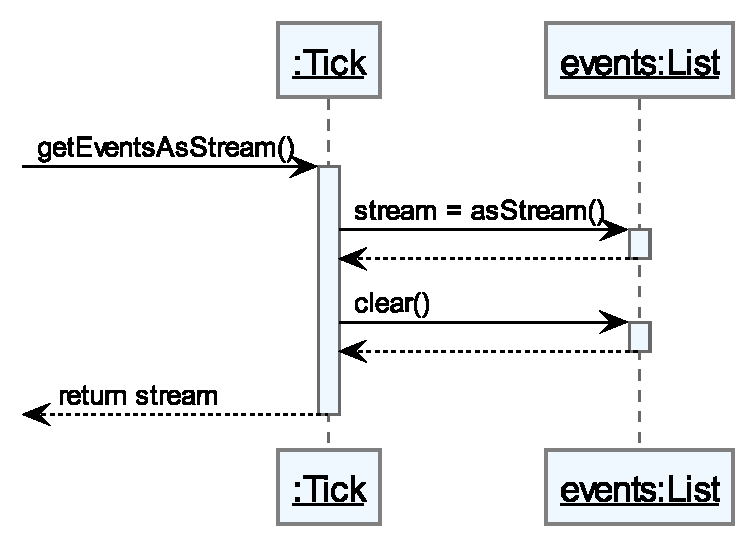
\includegraphics[width=0.5\linewidth]{Interface/Tick_getEventsAsStream.eps}
    \captionof{figure}{Tick.getEventsAsStream()}
\end{center}

\begin{center}
    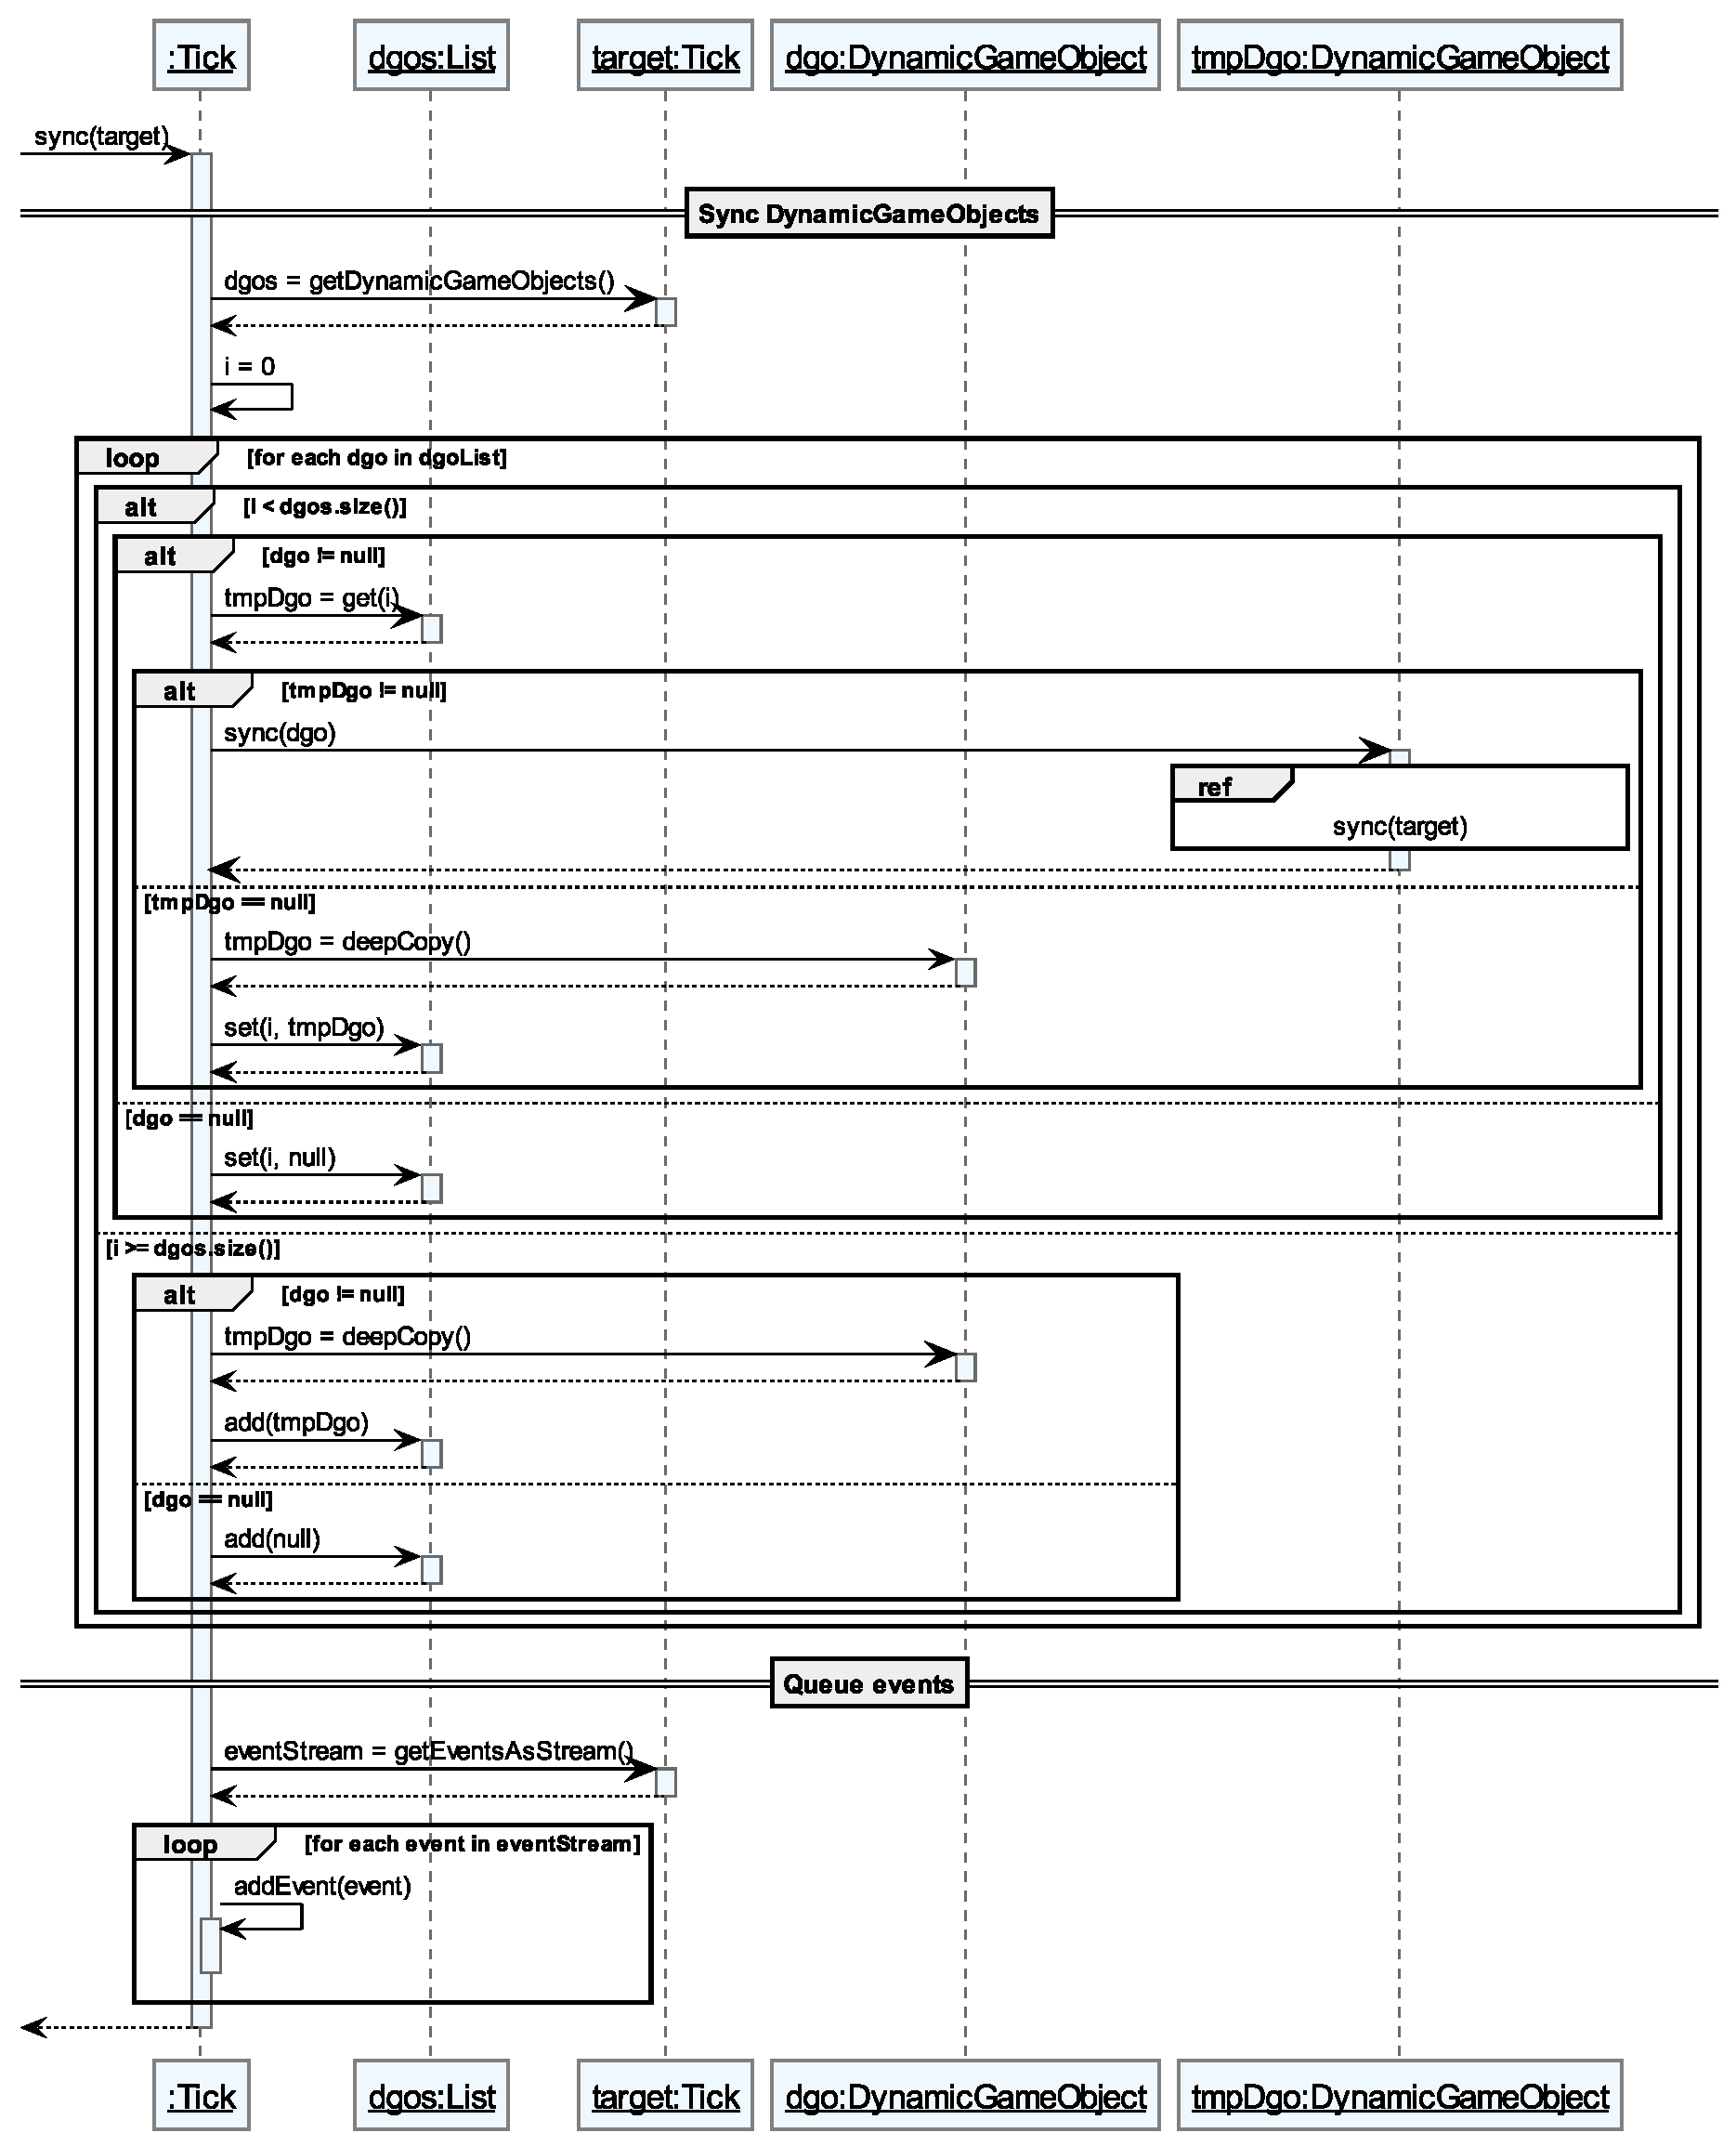
\includegraphics[width=\linewidth]{Interface/Tick_sync.eps}
    \captionof{figure}{Tick.sync()}
\end{center}

\subsubsection{tick.DynamicGameObject}
Die Funktionen sind analog zu den funktionen in \textit{tick.Tick}

\subsubsection{rendering.tick.TickProcessor}

\begin{center}
    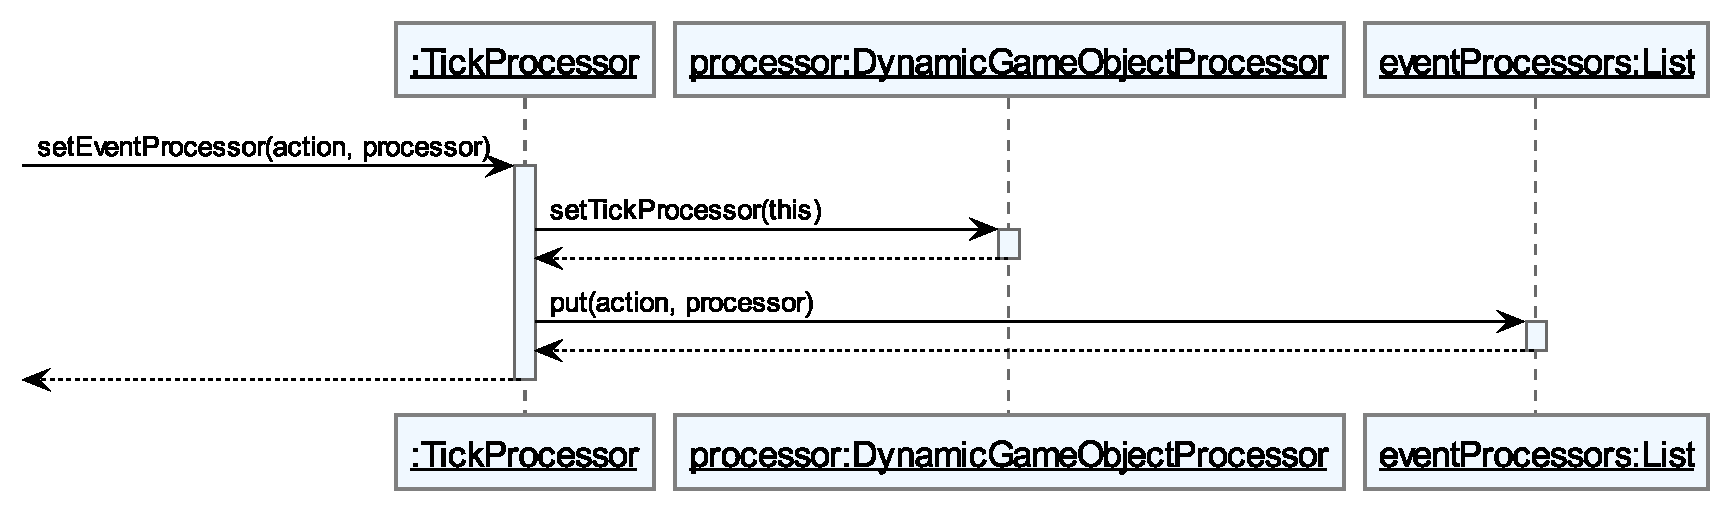
\includegraphics[width=\linewidth]{Interface/TickProcessor_setEventProcessor.eps}
    \captionof{figure}{TickProcessor.setEventProcessor()}
\end{center}

\begin{center}
    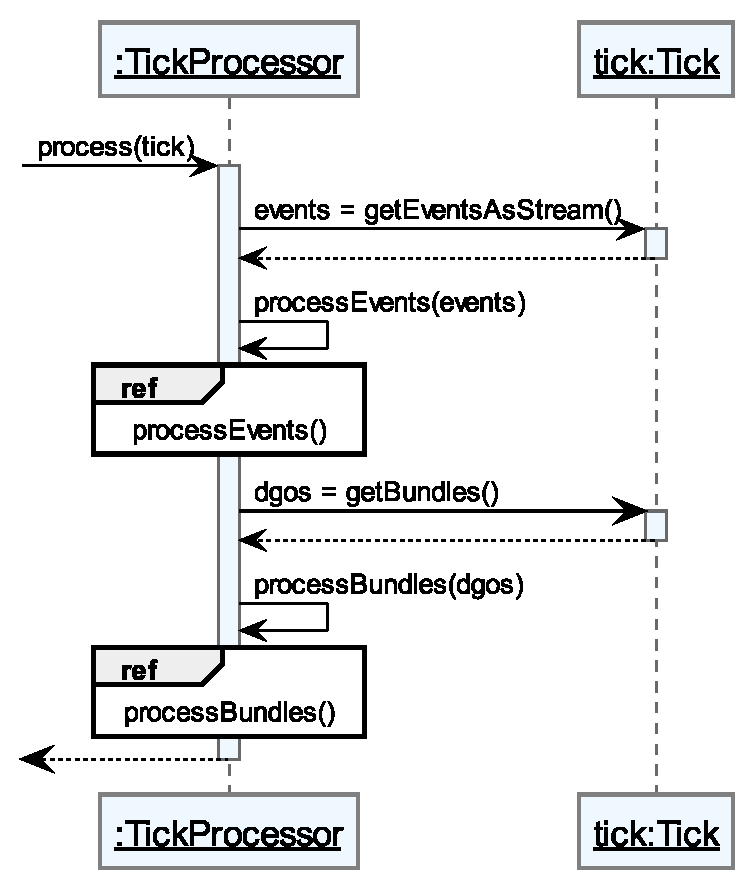
\includegraphics[width=0.5\linewidth]{Interface/TickProcessor_process.eps}
    \captionof{figure}{TickProcessor.process()}
\end{center}

\begin{center}
    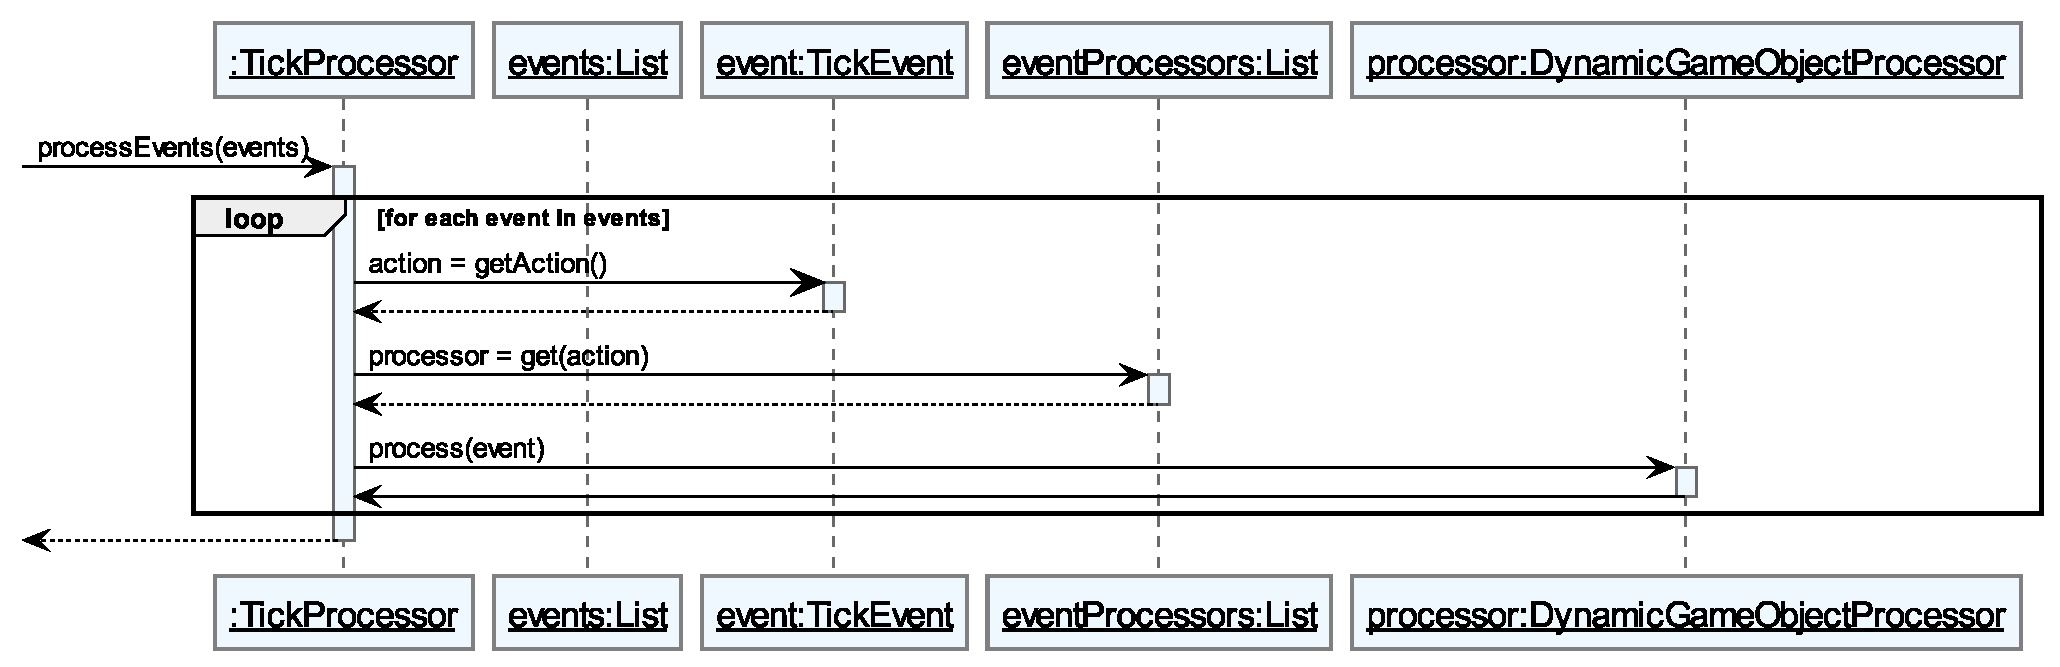
\includegraphics[width=\linewidth]{Interface/TickProcessor_processEvents.eps}
    \captionof{figure}{TickProcessor.processEvents()}
\end{center}

\begin{center}
    \centering
    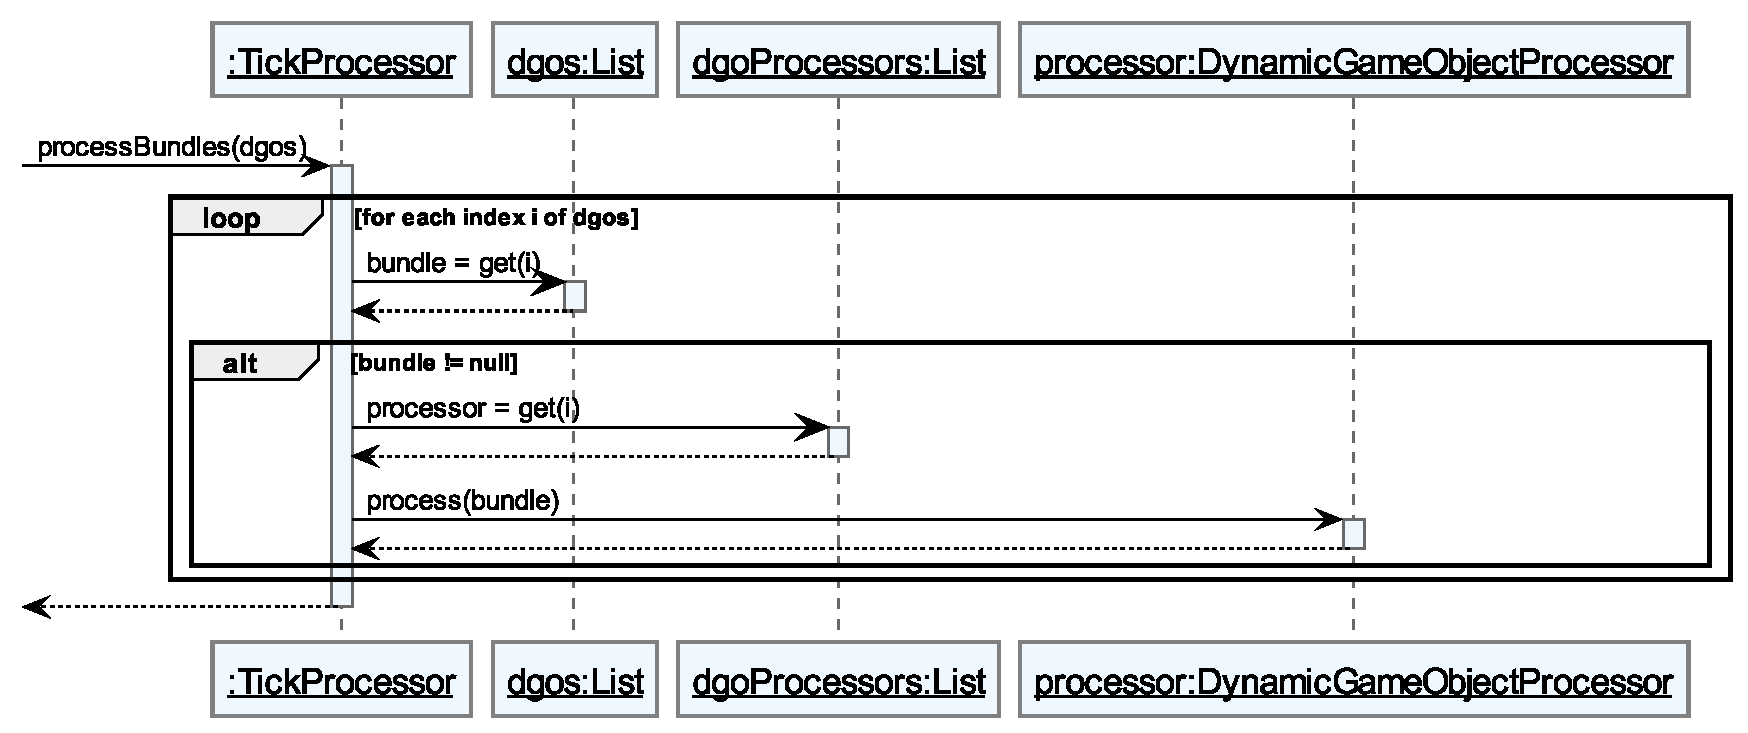
\includegraphics[width=\linewidth]{Interface/TickProcessor_processBundles.eps}
    \captionof{figure}{TickProcessor.processDynamicGameObjects()}
\end{center}

\subsubsection{rendering.tick.DynamicGameObjectProcessor}
Die Funktionen sind analog zu den funktionen in \textit{rendering.tick.TickProcessor}